\documentclass[12pt,a4paper]{article}

\usepackage[utf8]{inputenc}
\usepackage[T1]{fontenc}
\usepackage[spanish]{babel}
\usepackage{geometry}
\usepackage{enumitem}
\usepackage{booktabs}
\usepackage{graphicx}
\usepackage{amsmath}
\usepackage[hidelinks]{hyperref}
\usepackage{float}
\usepackage{parskip}
\usepackage{titlesec}
\usepackage{fancyhdr}

\geometry{margin=2.5cm}
\setlength{\headheight}{14pt}
\graphicspath{{../outputs/figures/semana4/}{outputs/figures/semana4/}{../}{./}{../docs/}}
\setlist[itemize]{itemsep=0.35em, topsep=0.35em}
\setlist[enumerate]{itemsep=0.35em, topsep=0.35em}

\pagestyle{fancy}
\fancyhf{}
\rhead{\small Informe Final --- PRY3-MD}
\lhead{\small Universidad del Valle de Guatemala}
\rfoot{\small \thepage}
\renewcommand{\headrulewidth}{0.4pt}
\renewcommand{\tablename}{Cuadro}

\begin{document}

% ── CARÁTULA ──────────────────────────────────────────────────────────────────
\begin{titlepage}
    \thispagestyle{empty}
    \centering
    \vspace*{0.4cm}

    \includegraphics[width=0.32\textwidth]{LogoUVG.png}\\[0.7cm]

    {\Large\bfseries UNIVERSIDAD DEL VALLE DE GUATEMALA}\\[0.3cm]
    {\large 1CC30743020261 --- Miner\'ia de Datos --- Secci\'on 30}\\[0.15cm]
    {\large Catedr\'atico: Luis Furlan}\\[1.4cm]

    \rule{\textwidth}{0.6pt}\\[0.4cm]
    {\LARGE\bfseries Informe Final}\\[0.25cm]
    {\large\bfseries Predicci\'on del Porcentaje de Uso de Internet\\[0.1cm]
    en Am\'erica Latina y el Caribe}\\[0.2cm]
    \rule{\textwidth}{0.6pt}\\[1.4cm]

    \begin{tabular}{ll}
        \textbf{Nombre}    & \textbf{Carnet} \\[0.35em]
        Roberto Barreda    & 23354 \\[0.2em]
        Javier Espa\~na    & 23361 \\[0.2em]
        Diego L\'opez      & 23747 \\[0.2em]
        \'Angel Esquit     & 23221 \\
    \end{tabular}\\[1.5cm]

    {\large Guatemala, 29 de mayo de 2026}
\end{titlepage}

% ── ÍNDICE ────────────────────────────────────────────────────────────────────
\tableofcontents
\newpage

% ── PROBLEMA ANALÍTICO ────────────────────────────────────────────────────────
\section{Problema anal\'itico}

El objetivo del proyecto fue cuantificar y predecir la \textbf{penetraci\'on de Internet} en pa\'ises de Am\'erica Latina y el Caribe, desagregada por pa\'is, a\~no y grupo etario. Entender c\'omo var\'ia el porcentaje de personas usuarias de Internet en funci\'on de estas tres dimensiones tiene valor directo para pol\'iticas p\'ublicas de inclusi\'on digital, ya que permite identificar brechas geogr\'aficas y generacionales con precisi\'on.

El problema se formul\'o como \textbf{regresi\'on supervisada}: la variable objetivo es continua (porcentaje de uso), y las entradas son pa\'is, a\~no y grupo etario. La unidad de an\'alisis es cada combinaci\'on pa\'is-a\~no-grupo, lo que convierte el problema en un panel de datos con estructura temporal y transversal.

% ── MARCO TEÓRICO ─────────────────────────────────────────────────────────────
\section{Marco te\'orico}

\subsection{Aprendizaje supervisado y regresi\'on}

El \textbf{aprendizaje supervisado} es una rama del machine learning en la que un algoritmo aprende una funci\'on de mapeo a partir de pares entrada-salida etiquetados. Cuando la variable objetivo es continua, el problema se denomina \textbf{regresi\'on}. El modelo busca minimizar un criterio de error sobre el conjunto de entrenamiento y generalizar a datos no vistos.

Las m\'etricas est\'andar en problemas de regresi\'on son el Error Absoluto Medio (MAE), la Ra\'iz del Error Cuadr\'atico Medio (RMSE) y el coeficiente de determinaci\'on ($R^2$). El MAE mide el error promedio en las mismas unidades que la variable objetivo; el RMSE penaliza m\'as los errores grandes; y $R^2$ cuantifica la proporci\'on de varianza explicada por el modelo.

\subsection{M\'etodos de ensamble}

Los \textbf{m\'etodos de ensamble} combinan m\'ultiples modelos base para obtener predicciones m\'as robustas. Existen dos estrategias principales:

\begin{itemize}
    \item \textbf{Bagging (Bootstrap Aggregating):} construye modelos independientes en paralelo sobre muestras con reemplazo y promedia sus predicciones. \textbf{Random Forest} es el ejemplo m\'as conocido.
    \item \textbf{Boosting:} construye modelos de forma secuencial, donde cada uno corrige los errores del anterior. \textbf{Gradient Boosting} entrena sucesivos \'arboles minimizando el gradiente de una funci\'on de p\'erdida, lo que le otorga alta capacidad expresiva.
\end{itemize}

\subsection{Validaci\'on cruzada temporal}

En problemas con componente temporal, el uso de una divisi\'on aleatoria entre entrenamiento y prueba puede producir \textbf{fuga de informaci\'on}: el modelo entrena sobre datos futuros y se eval\'ua en datos pasados, inflando artificialmente las m\'etricas. La \textbf{validaci\'on cruzada de ventana expandida} (expanding window cross-validation) resuelve esto: en cada fold, el entrenamiento incluye todos los datos hasta un punto $t$ y la validaci\'on se realiza sobre el per\'iodo $t+1$, simulando siempre una predicci\'on hacia el futuro.

\subsection{Datos de panel}

Un \textbf{panel de datos} combina dimensiones transversales (pa\'ises, grupos etarios) y una dimensi\'on temporal (a\~nos). Este tipo de estructura presenta retos espec\'ificos: autocorrelaci\'on temporal, heterogeneidad no observada entre unidades y posibles desfases en el efecto de las variables. La correcta preparaci\'on del panel para machine learning requiere codificar las identidades de cada unidad, construir variables temporales derivadas y respetar el orden cronol\'ogico en la validaci\'on.

% ── DATOS Y PREPARACIÓN ───────────────────────────────────────────────────────
\section{Datos y preparaci\'on}

El conjunto original proviene de \textbf{CEPALSTAT} y presenta observaciones para pa\'ises seleccionados de Am\'erica Latina y el Caribe, con cobertura desde 2000 hasta 2022. El an\'alisis exploratorio revel\'o tres hallazgos relevantes:

\begin{itemize}
    \item La adopci\'on de Internet crece con fuerza en el tiempo y muestra una tendencia no lineal.
    \item Existen diferencias marcadas entre pa\'ises, con algunos casos sistem\'aticamente por encima del resto.
    \item La brecha generacional es persistente: los grupos j\'ovenes tienen valores de uso mucho m\'as altos que los adultos mayores.
\end{itemize}

Para llevar los datos a un formato compatible con aprendizaje supervisado se aplic\'o una transformaci\'on que incluy\'o codificaci\'on de variables categ\'oricas (pa\'is y grupo etario) y creaci\'on de la variable derivada \texttt{years\_since\_2016}. El an\'alisis se restringi\'o al per\'iodo 2016--2022 por dos razones: la cobertura mejora de forma importante a partir de ese punto y el problema de predicci\'on se vuelve m\'as consistente al evitar el tramo m\'as ruidoso del panel.

La versi\'on final del dataset conserva: \texttt{pais}, \texttt{anio}, \texttt{years\_since\_2016}, \texttt{porcentaje\_internet} y variables dummy del grupo etario.

% ── METODOLOGÍA ───────────────────────────────────────────────────────────────
\section{Metodolog\'ia experimental}

\subsection{Secuencia de trabajo}

El proyecto se organiz\'o en cuatro etapas:

\begin{enumerate}
    \item \textbf{Exploraci\'on inicial:} caracterizaci\'on del comportamiento global, validaci\'on de cobertura y detecci\'on de patrones por pa\'is y grupo etario.
    \item \textbf{Transformaci\'on:} preparaci\'on del dataset para machine learning, con codificaci\'on de categor\'ias y creaci\'on de variables derivadas.
    \item \textbf{Modelado inicial:} comparaci\'on de regresi\'on lineal, Random Forest y Gradient Boosting como baselines.
    \item \textbf{Mejora y selecci\'on:} afinamiento de hiperpar\'ametros mediante Grid Search y validaci\'on cruzada temporal para elegir el modelo final.
\end{enumerate}

\subsection{Validaci\'on temporal}

Para evitar fuga de informaci\'on se us\'o una partici\'on temporal estricta. El entrenamiento se realiz\'o con datos de 2016--2020 y la prueba final se reserv\'o para 2021--2022. Sobre el conjunto de desarrollo se implement\'o una validaci\'on cruzada de ventana expandida con cuatro folds secuenciales, de modo que cada fold simulara la predicci\'on de un per\'iodo futuro.

\subsection{Modelos evaluados}

Se evaluaron cinco configuraciones:

\begin{itemize}
    \item Regresi\'on lineal como baseline simple.
    \item Random Forest como ensamble de referencia.
    \item Random Forest optimizado mediante Grid Search.
    \item Gradient Boosting como baseline no lineal.
    \item Gradient Boosting optimizado como modelo candidato final.
\end{itemize}

Las m\'etricas principales fueron MAE, RMSE y $R^2$, evaluadas tanto en validaci\'on cruzada como en el conjunto de prueba temporal.

% ── RESULTADOS ────────────────────────────────────────────────────────────────
\section{Resultados principales}

\subsection{Comparaci\'on de modelos}

El Cuadro~\ref{tab:comparacion} resume el desempe\~no de todos los modelos evaluados. El patr\'on es claro: la regresi\'on lineal no captura la no linealidad del problema, mientras que los ensambles de \'arboles reducen el error de forma importante. El mejor resultado lo obtuvo Gradient Boosting optimizado, que fue superior tanto en validaci\'on cruzada como en prueba final.

\begin{table}[H]
\centering
\caption{Comparaci\'on final de modelos}
\label{tab:comparacion}
\vspace{0.5em}
\resizebox{\textwidth}{!}{%
\begin{tabular}{lccccccc}
\toprule
\textbf{Modelo} & \textbf{Tipo} & \textbf{CV MAE (pp)} & \textbf{CV RMSE (pp)} & \textbf{CV $R^2$} & \textbf{Test MAE (pp)} & \textbf{Test RMSE (pp)} & \textbf{Test $R^2$} \\
\midrule
Regresi\'on lineal & Baseline & $12.60 \pm 1.98$ & $15.43 \pm 2.00$ & $0.617 \pm 0.053$ & $8.35$ & $10.60$ & $0.732$ \\
Random Forest & Baseline & $6.28 \pm 1.71$ & $8.06 \pm 2.61$ & $0.888 \pm 0.064$ & $5.81$ & $6.92$ & $0.886$ \\
RF optimizado & Optimizado & $6.26 \pm 1.64$ & $8.14 \pm 2.62$ & $0.886 \pm 0.064$ & $5.67$ & $6.76$ & $0.891$ \\
Gradient Boosting & Baseline & $6.21 \pm 1.16$ & $8.32 \pm 2.26$ & $0.882 \pm 0.055$ & $5.48$ & $6.92$ & $0.886$ \\
\textbf{GB optimizado} & \textbf{Optimizado} & \textbf{$5.33 \pm 1.17$} & \textbf{$7.51 \pm 2.71$} & \textbf{$0.900 \pm 0.063$} & \textbf{$4.97$} & \textbf{$6.11$} & \textbf{$0.911$} \\
\bottomrule
\end{tabular}
}
\end{table}

\subsection{Hiperpar\'ametros seleccionados}

Los mejores hiperpar\'ametros encontrados mediante Grid Search se presentan en el Cuadro~\ref{tab:hiperparametros}.

\begin{table}[H]
\centering
\caption{Hiperpar\'ametros \'optimos por modelo}
\label{tab:hiperparametros}
\vspace{0.4em}
\begin{tabular}{lll}
\toprule
\textbf{Par\'ametro}    & \textbf{Random Forest} & \textbf{Gradient Boosting} \\
\midrule
\texttt{n\_estimators}  & 200   & 200  \\
\texttt{max\_depth}     & None  & 5    \\
\texttt{learning\_rate} & ---   & 0.2  \\
\texttt{max\_features}  & 1.0   & ---  \\
\texttt{min\_samples\_leaf} & 1 & 2    \\
\bottomrule
\end{tabular}
\end{table}

La ganancia del ajuste fue baja en Random Forest y alta en Gradient Boosting, lo que sugiere que la arquitectura de boosting ten\'ia m\'as capacidad de aprovechar la sintonizaci\'on fina.

\subsection{Visualizaciones}

\begin{figure}[H]
    \centering
    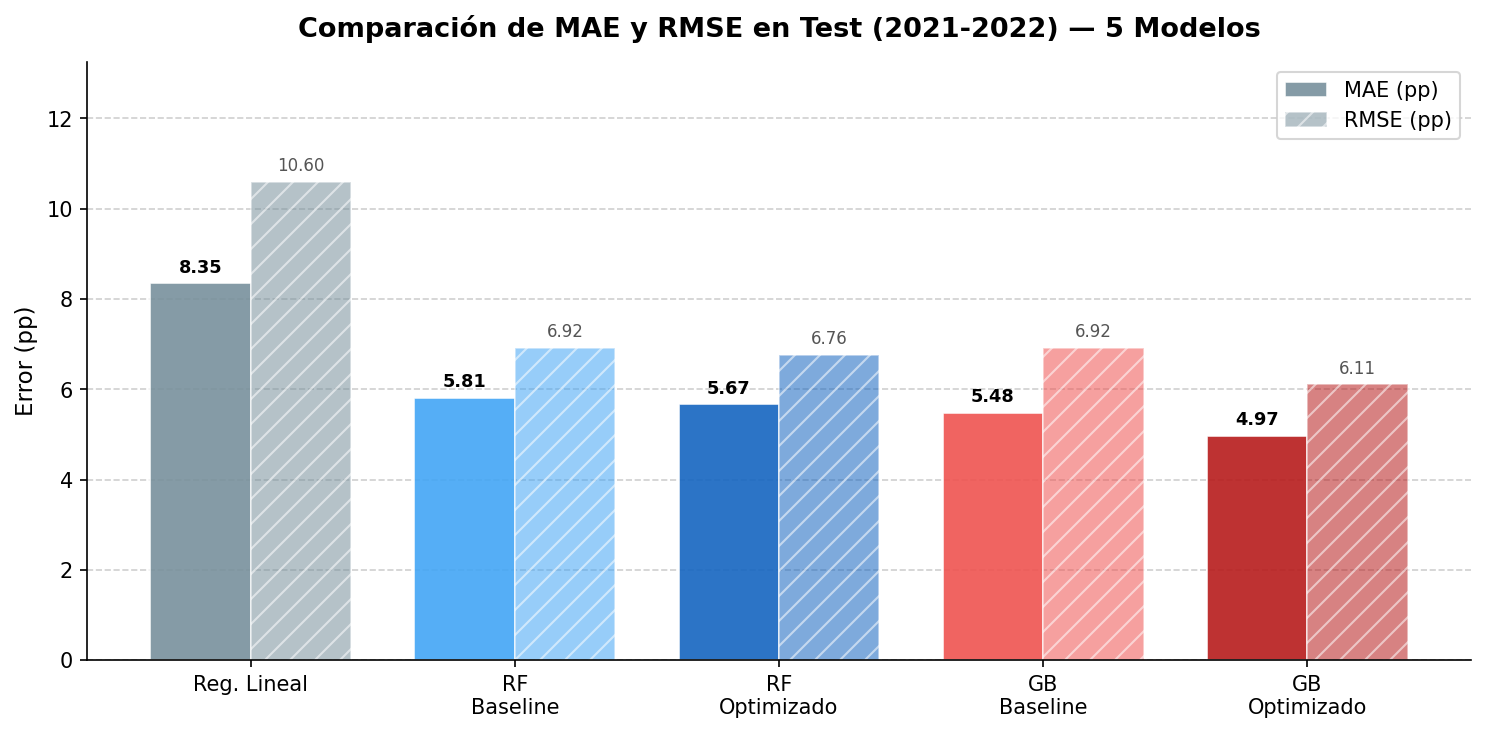
\includegraphics[width=0.85\textwidth]{fig1_comparacion_mae_rmse.png}
    \caption{Comparaci\'on de MAE y RMSE entre los modelos evaluados.}
    \label{fig:mae_rmse}
\end{figure}

\begin{figure}[H]
    \centering
    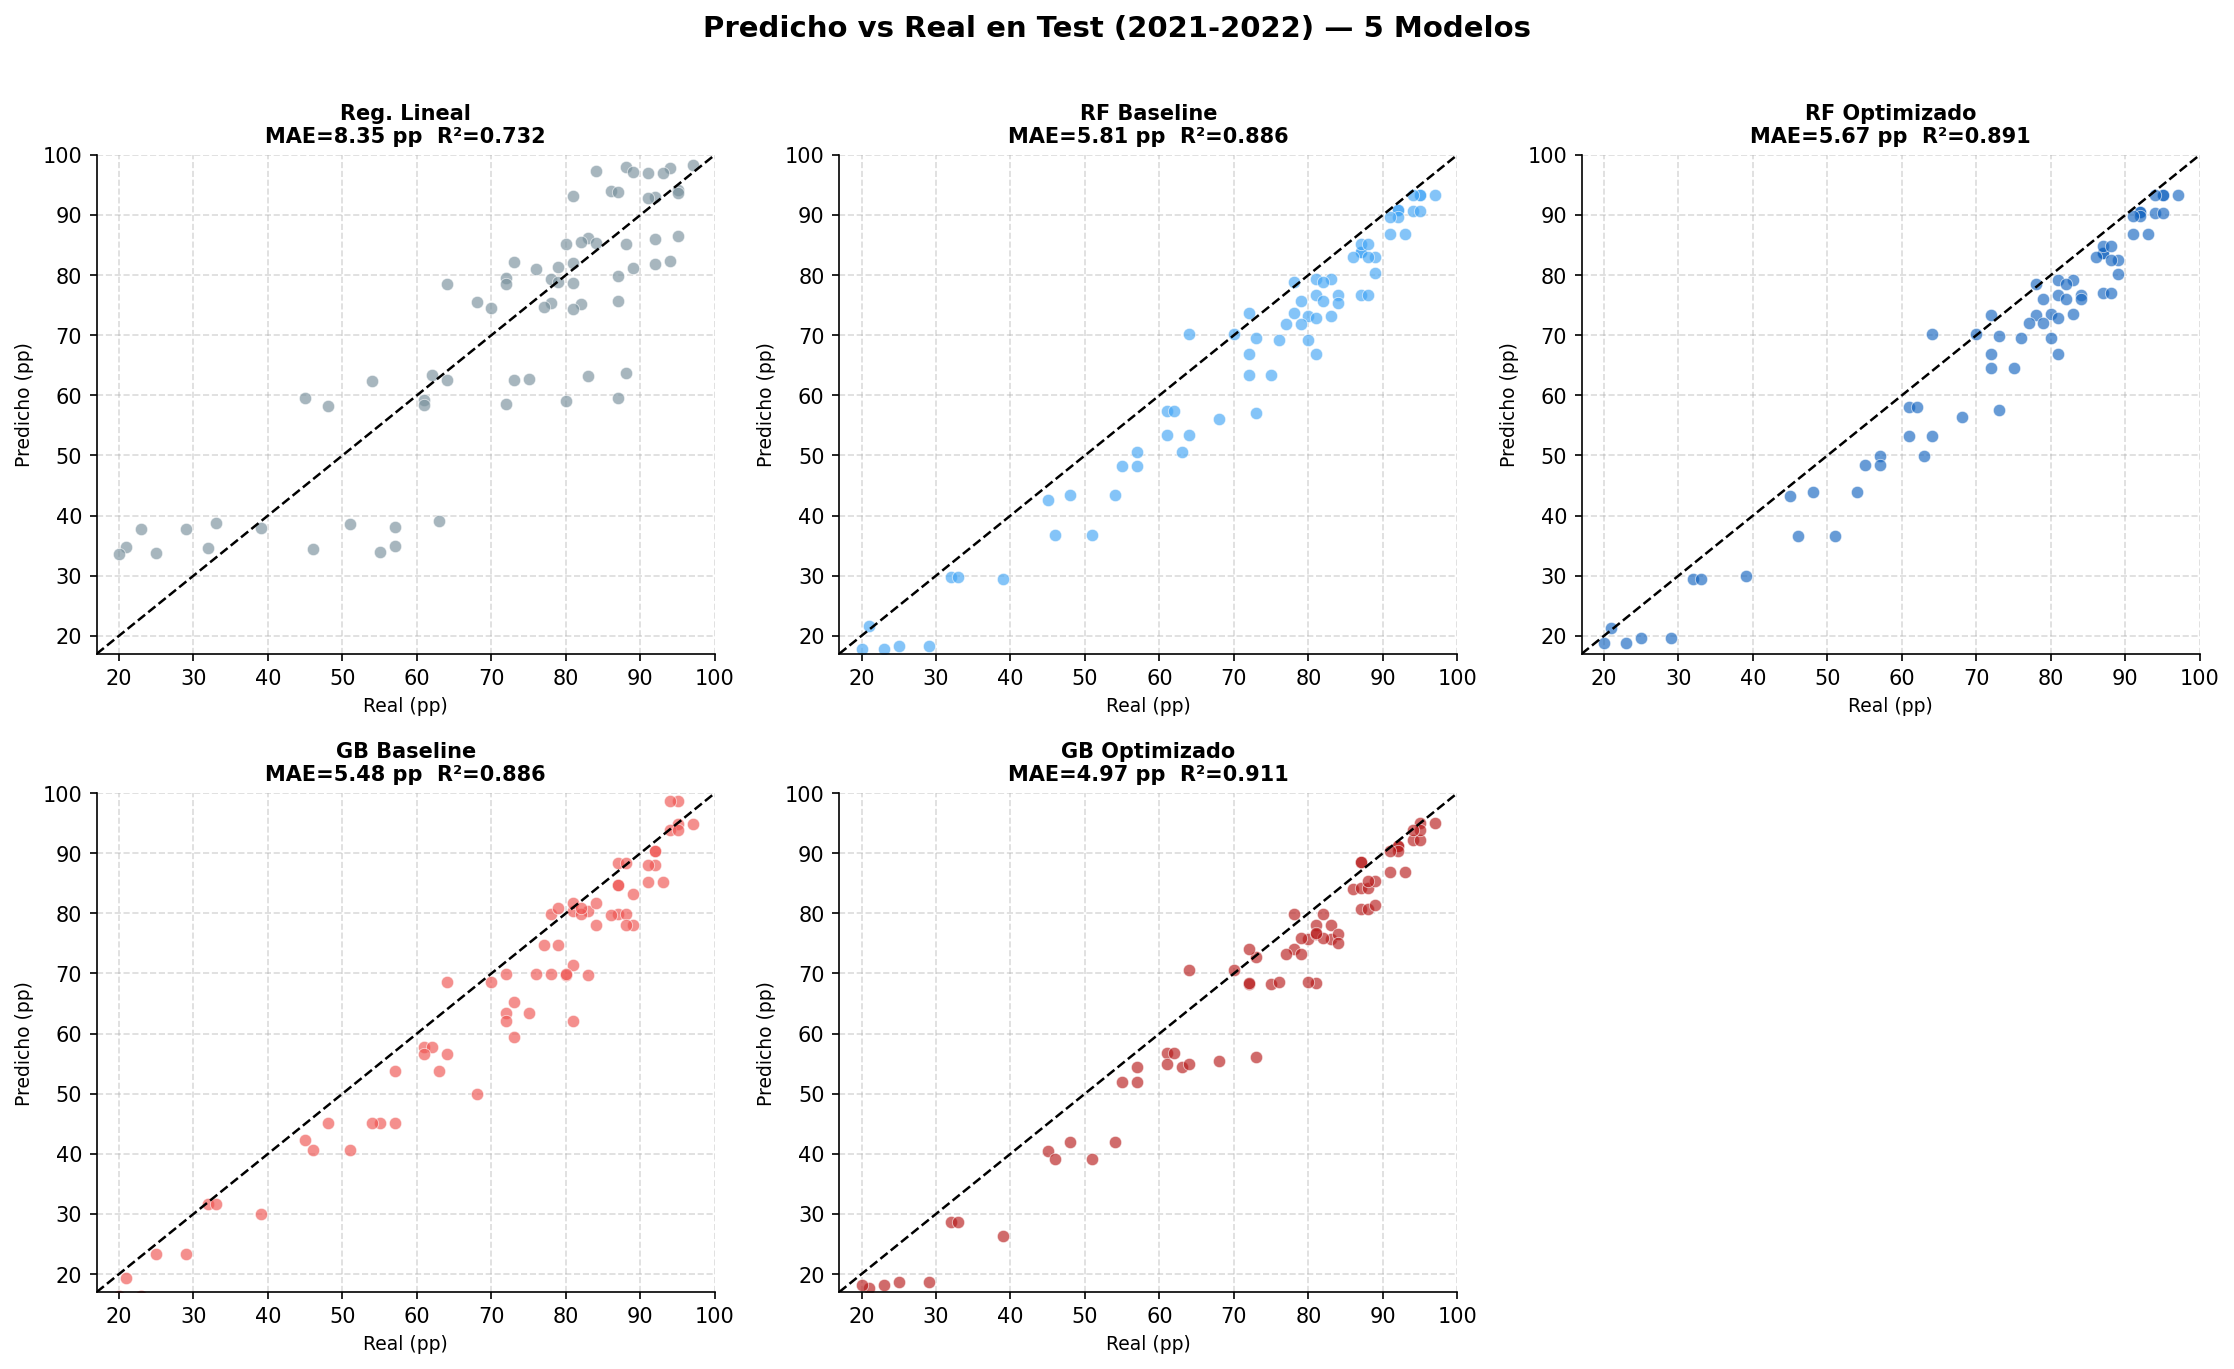
\includegraphics[width=0.85\textwidth]{fig2_predicho_vs_real.png}
    \caption{Relaci\'on entre valores reales y predichos por el modelo final.}
    \label{fig:pred_real}
\end{figure}

\begin{figure}[H]
    \centering
    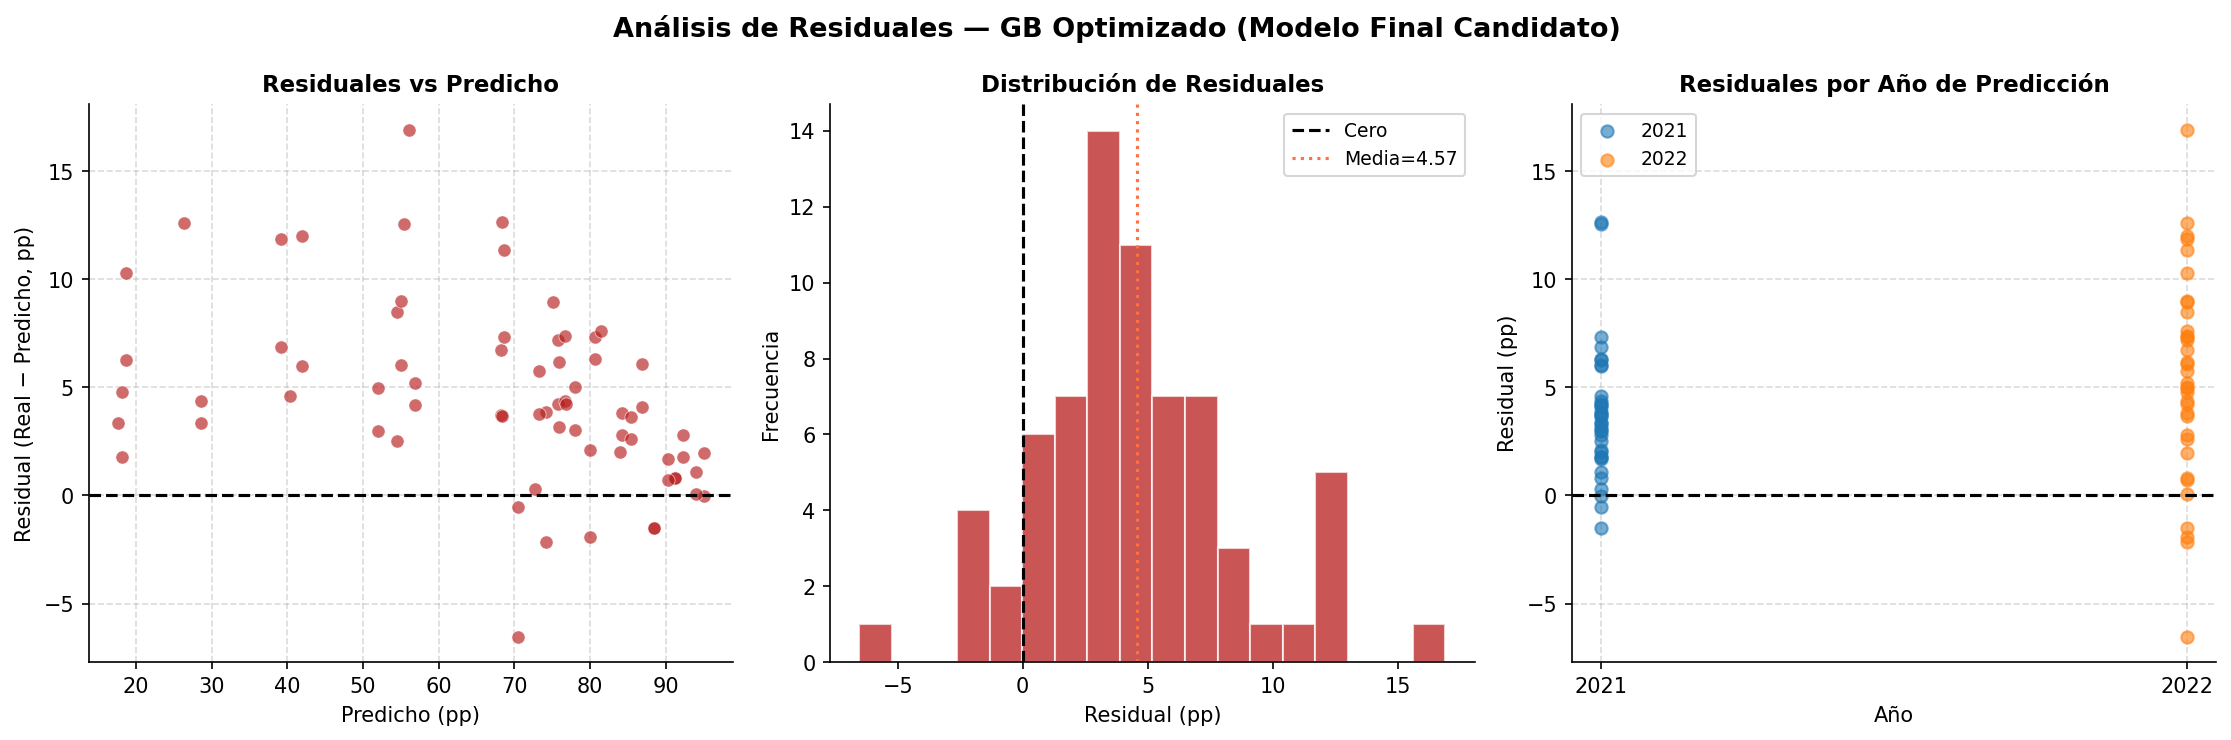
\includegraphics[width=0.85\textwidth]{fig3_residuales_gb_opt.png}
    \caption{Distribuci\'on de residuales del Gradient Boosting optimizado.}
    \label{fig:residuales}
\end{figure}

\begin{figure}[H]
    \centering
    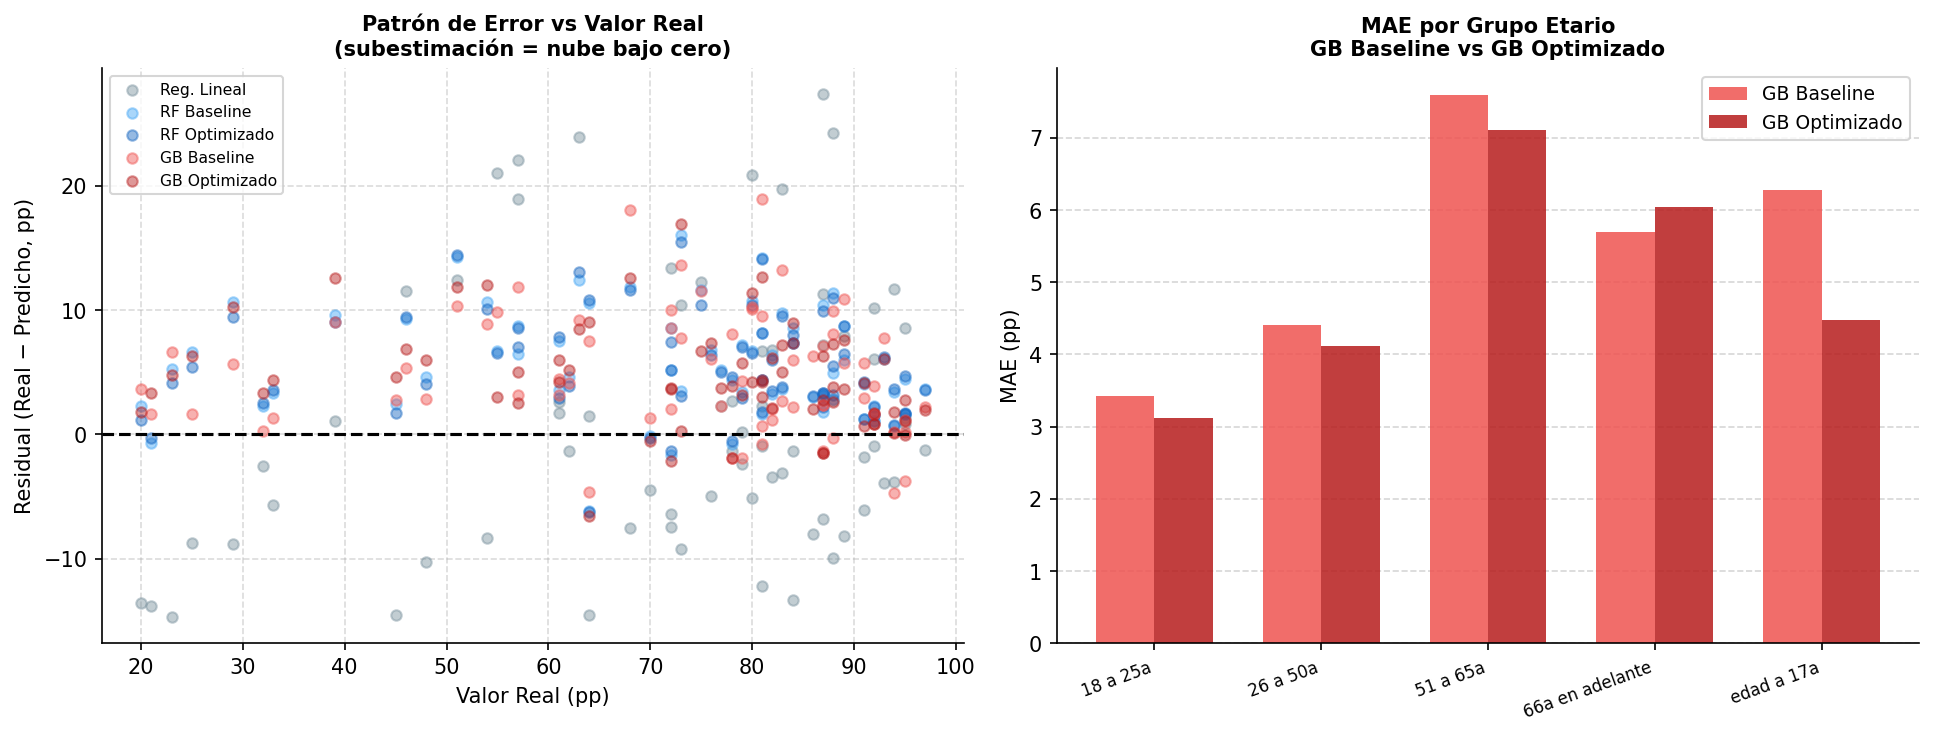
\includegraphics[width=0.85\textwidth]{fig4_subestimacion_y_grupos.png}
    \caption{Patr\'on de subestimaci\'on por grupos etarios y pa\'ises.}
    \label{fig:subestimacion}
\end{figure}

% ── ANÁLISIS DE ERRORES ───────────────────────────────────────────────────────
\section{An\'alisis de errores del modelo}

\subsection{Comportamiento global del modelo final}

El Gradient Boosting optimizado obtuvo un MAE de 4.97 puntos porcentuales en prueba y un $R^2$ de 0.911, lo que indica que el modelo explica bien la variabilidad entre pa\'ises y grupos etarios. Sin embargo, el error no es completamente aleatorio. El an\'alisis de residuales mostr\'o una media residual positiva de $+4.57$ pp, mediana de $+4.14$ pp, desviaci\'on est\'andar de $4.06$ pp y subestimaci\'on en el 90\,\% de los casos.

\subsection{Interpretaci\'on de la subestimaci\'on}

El sesgo sistem\'atico se explica por la tensi\'on entre la historia observada y el contexto futuro. El entrenamiento cubri\'o 2016--2020, mientras que la prueba incluy\'o 2021--2022, per\'iodo en el que se registr\'o una adopci\'on digital m\'as acelerada. Los modelos basados en \'arboles interpolan bien dentro del rango de entrenamiento pero no extrapolan con facilidad cuando el futuro presenta una aceleraci\'on estructural. Esta lectura evita confundir sesgo estructural con ruido aleatorio.

\subsection{Desempe\~no por grupos y pa\'ises}

Los errores no se distribuyen de manera homog\'enea. Los grupos etarios m\'as altos (especialmente \emph{66 a\~nos en adelante}) presentan mayor dispersi\'on, mientras que los grupos j\'ovenes son m\'as estables. A nivel geogr\'afico, el error fue m\'as bajo en pa\'ises con trayectorias estables como Argentina, Costa Rica y Colombia, y m\'as alto en pa\'ises con din\'amicas m\'as abruptas como Panam\'a y Per\'u.

% ── CONCLUSIONES ──────────────────────────────────────────────────────────────
\section{Conclusiones}

\begin{enumerate}
    \item La penetraci\'on de Internet en Am\'erica Latina y el Caribe creci\'o de forma sostenida entre 2016 y 2022, con una aceleraci\'on notable a partir de 2020 impulsada por la pandemia.
    \item Existe una brecha generacional persistente y amplia: los grupos j\'ovenes (15--24 a\~nos) registran tasas de uso consistentemente superiores a las de los adultos mayores (66 a\~nos en adelante) en todos los pa\'ises analizados.
    \item Las diferencias entre pa\'ises son significativas y estables en el tiempo; Argentina, Costa Rica y Colombia presentan los niveles de penetraci\'on m\'as altos, mientras que otros pa\'ises mantienen rezagos estructurales.
    \item La brecha digital generacional no se cierra proporcionalmente con el tiempo: los grupos mayores acumulan un atraso relativo que se mantiene incluso en pa\'ises con mayor desarrollo digital.
    \item El a\~no, el pa\'is y el grupo etario son los tres factores que explican la mayor parte de la variaci\'on en la penetraci\'on de Internet, confirmando que la inclusi\'on digital es un fen\'omeno multidimensional.
    \item La pandemia de COVID-19 introdujo una discontinuidad estructural en la adopci\'on digital de la regi\'on: la aceleraci\'on registrada en 2021--2022 excede los patrones hist\'oricos y no es predecible a partir de datos anteriores a 2020.
    \item Los pa\'ises con trayectorias m\'as abruptas o irregulares (como Panam\'a y Per\'u) evidencian que la penetraci\'on de Internet no sigue un patr\'on uniforme en la regi\'on, sino que depende de factores econ\'omicos e institucionales propios de cada contexto nacional.
    \item Para cerrar efectivamente las brechas digitales en LATAM se requieren pol\'iticas diferenciadas: intervenciones espec\'ificas para adultos mayores y estrategias nacionales que atiendan las condiciones particulares de cada pa\'is.
\end{enumerate}

% ── ANEXOS ────────────────────────────────────────────────────────────────────
\appendix
\section{Repositorio de c\'odigo}

El c\'odigo fuente del proyecto, incluyendo los notebooks de exploraci\'on, transformaci\'on, modelado y evaluaci\'on, se encuentra disponible en el siguiente repositorio de GitHub:

\begin{center}
    \href{https://github.com/dlop6/PRY3-MD}{\texttt{https://github.com/dlop6/PRY3-MD}}
\end{center}

El repositorio contiene la estructura completa del proyecto: datos de entrada, notebooks por etapa, figuras generadas y este informe en formato \LaTeX.

\end{document}
